\begin{frame}
    \frametitle{a 地理作業}

    自己查

\end{frame}


\begin{frame}
    \frametitle{觀察資料}
    尋找正確的模型有一些作法
    \begin{enumerate}
        \item 從既有文獻。適合短時間畢業。
        \item 觀察散佈圖,看圖說故事。數據驅動(Data driven)的分析。適合初步了解數據。
        \item 從一些結構性的關係(structural relation)推倒變數之間的關聯。較適合處理有嚴重內生性的變數關係。
    \end{enumerate}
\end{frame}

\begin{frame}[plain]
    \code{scatter pfood totexp}
    \begin{figure}
        \includegraphics[width=0.8\textwidth]{../Results/Q4_11_simple_scatter.eps}
    \end{figure}
\end{frame}

\begin{frame}
    \frametitle{totexp 變數好像不太「正常」}
    繪製長條圖

    \code{hist totexp, name(hist\_of\_totexp)}

    匯出圖檔

    \code{graph export "Q4\_11\_hist\_of\_totexp.eps", name(hist\_of\_totexp)}

    \begin{figure}
        \includegraphics[height=0.5\textheight]{../Results/Q4_11_hist_of_totexp.eps}
    \end{figure}
\end{frame}

\begin{frame}
    \frametitle{如果取對數?}

    \begin{figure}
        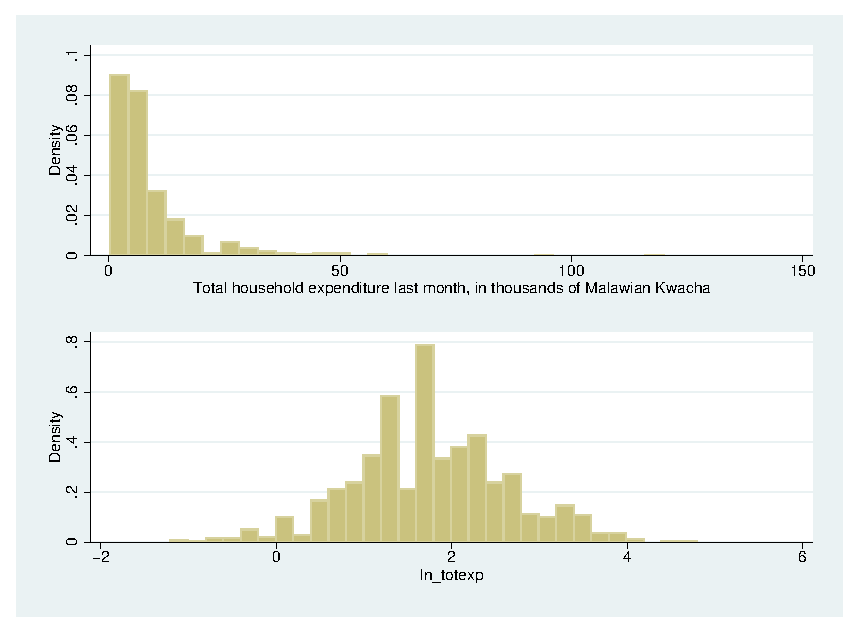
\includegraphics[height=0.8\textheight]{../Results/Q4_11_compare_totexp.eps}
    \end{figure}

    我們決定以$TOTEXP$的對數來處理資料
\end{frame}

\begin{frame}[fragile, allowframebreaks]
    \frametitle{b, c}
    b, c 小提上次助教課已做過,不再重複
    \begin{lstlisting}
eststo est_b: reg pfood ln_totexp
esttab, ci
    \end{lstlisting}

    \begin{lstlisting}
        capture program drop elas

// program 函數名稱
program elas
    args total_ex est_name

    qui estimates restore `est_name'    
    nlcom Elasticity: (_b[_cons] + _b[ln_totexp]*(log(`total_ex') +1) ) ///
        /(_b[_cons] + _b[ln_totexp]*log(`total_ex') )   ///
        , noheader
end

quietly sum totexp, detail
scalar total_ex_p5 = r(p5)
scalar total_ex_p75 = r(p75)

elas total_ex_p5 est_b
elas total_ex_p75 est_b
    \end{lstlisting}
\end{frame}

\begin{frame}
    \frametitle{D}
    從 (b) 小題中的模型計算殘差。建造這些殘差的直方圖,並針對 $\ln(TOTEXP)$繪製他們。有沒有明顯的模式?找到殘差的樣本偏態與峰態,以 $1\%$顯著水準進行 Jarque-Bera 檢定。
\end{frame}

\begin{frame}
    \frametitle{b, d, e, f, g, h在做什麼?}
    \begin{itemize}
        \item b, e, g 提出各種模型
        \item d, f, h 在進行殘差項診斷(Residual Diagnosis)
    \end{itemize}

    線性迴歸模型要能正確地假設,包含
    \begin{block}{OLS其中三項假設}
        \begin{enumerate}
            \item 外生性假設:$E[e_i \given X_i] = 0$
            \item 獨立:$Cov(e_i, e_j \given X_i) = 0$
            \item (選擇性)殘差分佈符合常態:$e_i \given X_i  \sim \mathcal{N}(0, \sigma^2)$
        \end{enumerate}
    \end{block}

    如果樣本數不夠大,要做統計檢定就一定需要透過殘差項符合常態分佈的假設,否則出來的不會是 t檢定,此時判斷 p-value 也就毫無意義。
\end{frame}